\section{Experimental Design and Methodology}\label{sec:exp}
To evaluate how decentralized negotiation mechanisms perform under the physical, informational, strategic, and communication constraints formulated in Section~\ref{sec:problem}, this section develops a modular negotiation protocol, a nine-policy benchmark taxonomy, and a reproducible dual-simulator experimental suite, organized around RQ1--RQ4.

\subsection{Decentralized Negotiation Protocol and Safeguards}\label{sec:proto}
All communicating policies execute inside a shared five-mode agent state machine (\texttt{CRUISE}, \texttt{NEGOTIATE}, \texttt{YIELD}, \texttt{PROCEED}, \texttt{DONE}) stepped at $20$\,Hz ($\Delta t = 0.05$\,s; Fig.~\ref{fig:proto}a).

\begin{figure*}[!t]\centering
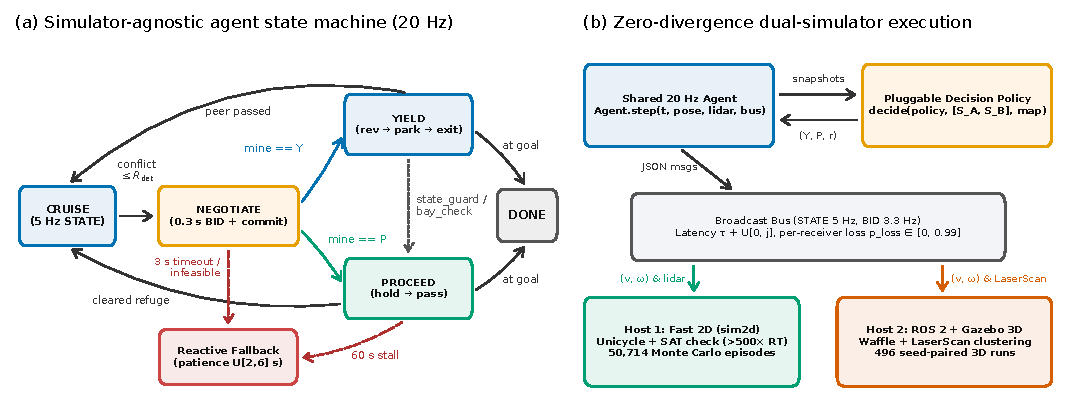
\includegraphics[width=1\textwidth]{Images/protocol.pdf}
\caption{Decentralized negotiation protocol and dual-simulator execution architecture. (a) Simulator-agnostic $20$\,Hz agent state machine showing nominal transitions (solid), timeout/infeasibility reactive fallbacks (dashed red), and lossy-channel yield-abort guards (dotted gray). (b) Zero-code-divergence execution architecture connecting the shared $20$\,Hz \texttt{Agent} controller and pluggable decision policy to both the fast 2D unicycle simulator (\texttt{sim2d}) and 3D ROS~2 Jazzy / Gazebo Harmonic.}
\label{fig:proto}
\end{figure*}

\subsubsection{Conflict Detection and Deterministic Snapshot Resolution}
While in \texttt{CRUISE}, robots broadcast 5\,Hz \texttt{STATE} beacons containing their pose, velocity, control mode, and corridor entry time (considered fresh for 1.0\,s). A conflict is triggered when a peer's beacon indicates an opposing robot within $R_{\mathrm{det}} = 6.0$\,m. Setting $R_{\mathrm{det}}$ beyond the 3.5\,m Lidar range ensures negotiation starts before either vehicle drives past a usable refuge.
Upon detection, each robot freezes its state into a kinematic \texttt{Snapshot} $S_i$ (pose, speed bounds, urgency, and payload status) and broadcasts it in a \texttt{BID} packet retransmitted every $0.3$\,s. Because each policy is a deterministic function of the sorted snapshot pair $(S_A, S_B)$ and the shared map, both robots independently compute the exact same \texttt{(yielder, proceeder, refuge)} assignment locally without requiring an extra handshake message.

\subsubsection{Lossy-Channel Safeguards and Liveness Fallbacks} 
Under severe packet drops or latency, robots may receive delayed messages and compute conflicting decisions. To prevent inconsistent execution, the protocol implements three switchable safeguards.
\begin{itemize}
\item \emph{Commit handshake (\texttt{commit}):} Robots attach their planned decision to outgoing \texttt{BID}s and wait for mutual confirmation. If decisions disagree, the lower-ID robot's choice takes precedence; unconfirmed decisions expire after 3.0\,s.
\item \emph{State guard (\texttt{state\_guard}):} A yielding robot monitors incoming peer \texttt{STATE} beacons and aborts its maneuver (switching to \texttt{PROCEED}) if the peer is also yielding to it or heading into the same bay.
\item \emph{Lidar bay check (\texttt{bay\_check}):} Bays with Lidar returns within 0.45\,m of the parking spot are treated as occupied during planning. If an en-route yielder detects a peer inside its target bay, it aborts and proceeds.
\end{itemize}
During execution, a proceeding robot advances only once \texttt{STATE} beacons or Lidar confirm the yielder is off-lane (renegotiating if the yielder continues cruising toward it). Similarly, a parked yielder exits once peer \texttt{STATE} confirms passage. If packet loss renders \texttt{STATE} stale, the yielder exits when Lidar confirms the peer has passed, or after a randomized hold $U[6,12]$\,s once the lane is clear.
To guarantee liveness under communication blackouts or deadlocks, robots fall back to reactive backoff when (i)~no peer \texttt{BID} arrives within $\tau_{\mathrm{neg}} = 3.0$\,s, (ii)~a proceeding robot stalls for $\tau_{\mathrm{proc}} = 60.0$\,s, or (iii)~neither robot has a feasible refuge ($\mathcal{F}=\emptyset$), triggering a 10.0\,s backoff. Receiving a valid peer \texttt{BID} at any time immediately resumes negotiation.

\subsubsection{Map-Uncertainty and Multi-Robot Extensions} 
Five protocol extensions address incomplete maps and multi-robot interactions. For map uncertainty, three extensions are included, namely, 
(i)~\texttt{share\_map} attaches known bay IDs to every \texttt{BID} so peers merge their maps before planning; 
(ii)~\texttt{explore} starts robots knowing only end rooms and discovers bays via Lidar within 3.5\,m (optionally gating map exchange on visual peer detection via \texttt{share\_on\_detect}, or pausing decisions up to 15.0\,s to await peer maps via \texttt{hold\_for\_map}); and 
(iii)~\texttt{refuge\_blocked} cross-checks Lidar returns inside bays against peer \texttt{STATE} beacons, broadcasting unmapped physical obstacles as blocked rather than mistaking them for parked robots. 
For multi-robot topologies, two rules are added, namely, 
(iv)~convoy \texttt{make\_room} instructs a trailing follower to back into an upstream bay if it blocks its reversing leader; and 
(v)~T-junction \texttt{goal\_wait} directs a robot whose branch destination is occupied to wait off-lane in an upstream bay rather than blocking the main corridor.

\subsection{Evaluated Coordination Policies}\label{sec:pol}
Table~\ref{tab:taxonomy} summarizes the nine policies evaluated across the benchmark studies. All negotiating policies map the frozen snapshot pair $(S_A, S_B)$ to a yielder $Y \in \{A, B\}$ and feasible refuge $r \in \mathcal{F}(Y, P)$.

\subsubsection{Non-Communicating, Lock, and Heuristic Rulebook Policies}
\texttt{reactive} (R) uses no communication; when Lidar detects an oncoming peer within braking distance, the robot stops, waits a random patience duration $U[2,6]$\,s to break symmetry, and reverses into the nearest refuge behind it if still blocked.
\texttt{reservation} (S) emulates first-come, first-served (FCFS) industrial zone control~\cite{fanti2002event} via \texttt{STATE} beacons; a robot outside the corridor ($[0,L]$) waits in its staging room whenever an opposing vehicle is already inside the aisle (falling back to \texttt{rules\_default} if both enter simultaneously).
\texttt{fixed\_priority} (F) is a static rule where the higher-ID robot always yields into its best feasible refuge $r^\ast$ unless no refuge is available ($\mathcal{F}=\emptyset$).
\texttt{rules\_default} (D) applies an ordered six-tier etiquette~\cite{kato1992coordinating,highwaycode} evaluated sequentially, checking 
(1)~refuge availability (if only one robot has a feasible refuge $\mathcal{F} \neq \emptyset$, it yields); 
(2)~task urgency (if $|u_A - u_B| \ge 0.5$, the less urgent robot yields); 
(3)~payload status (an unloaded robot yields to a loaded one); 
(4)~corridor seniority (the later entrant by $\ge 1.0$\,s yields); 
(5)~nearby refuge (if only one robot has a refuge within 2.0\,m behind it, it yields); and 
(6)~lower-ID tie-break. 
\texttt{rules\_proximity} (P) modifies this hierarchy by prioritizing geometry ahead of seniority, such that whichever robot is closer to its feasible refuge (by $\ge 0.1$\,m) yields immediately after checking payload.

\begin{table*}[!t]\centering
\caption{Taxonomy of benchmarked corridor coordination policies across communication, information inputs, model assumptions, and strategic properties.}
\label{tab:taxonomy}
{\footnotesize\setlength{\tabcolsep}{2.9pt}
\begin{tabular}{@{}llcccc>{\raggedright\arraybackslash}p{0.190\textwidth}@{}}\toprule
Policy (Code) & Family & Comms & State Inputs Used & Motion Model & Incentive Prop. & Multi-Robot / Map Scope \\\midrule
\texttt{reactive} (R) & Local sensor backoff & None & $3.5$\,m Lidar proximity & None & N/A & Pairwise/local; patience $U[2,6]$\,s \\
\texttt{reservation} (S) & Corridor mutex lock & \texttt{STATE} & Occupancy, $t_{\mathrm{enter}}$ & None & First-in wins & Corridor FCFS; rulebook inside-tie \\
\texttt{fixed\_priority} (F) & Static social law & \texttt{STATE}+\texttt{BID} & Robot ID, feasibility & Feasibility only & Non-manipulable$^\dagger$ & Pairwise + \texttt{make\_room} / \texttt{goal\_wait} \\
\texttt{rules\_default} (D) & Lexicographic rules & \texttt{STATE}+\texttt{BID} & $u_i$, load, $t_{\mathrm{enter}}$, bay $\le 2$\,m & Feasibility only & Non-manipulable$^\dagger$ & Ordered 6-rule industrial etiquette \\
\texttt{rules\_proximity} (P) & Geometric rulebook & \texttt{STATE}+\texttt{BID} & Nearest-bay $|x_r - x_i|$, D & Refuge distance & Pose-dependent & Closest-refuge ahead of seniority \\
\texttt{learned} (L) & Tabular classifier & \texttt{STATE}+\texttt{BID} & Binned bay dist., $u_i$, load & Offline sim table & Co-op assumed & 93 states; unseen $\to$ fixed priority \\
\cb\ (C) & Kinematic auction & \texttt{STATE}+\texttt{BID} & Full \texttt{Snapshot}, $u_i$ & Constant-speed & Manipulable & Pairwise social-cost minimization \\
\gb\ (G) & Convoy auction & \texttt{STATE}+\texttt{BID} & Group \texttt{Snapshot}s & Side-level sum & Co-op assumed & Distinct bays across convoy group \\
\texttt{clarke} (V) & VCG mechanism & \texttt{STATE}+\texttt{BID} & Cost vectors $b_i(o)$ & Constant-speed & DSIC (unilat.)$^\ddagger$ & Externality payment to fleet bank \\\bottomrule
\end{tabular}}\\[2pt]
{\footnotesize $^\dagger$Non-manipulable with respect to cost bids; physical state claims ($u_i$, load, known bays) are assumed authentic. $^\ddagger$Dominant-strategy incentive compatible for unilateral cost scaling under the shared kinematic model; runs a budget surplus and does not prevent joint shading or bay-set omission.}
\end{table*}

\subsubsection{Kinematic Cost Bidding (\cb) and Convoy Group Bidding (\gb)}
Under \cb\ (C), robots select the yielder that minimizes predicted urgency-weighted social delay using equation \eqref{eq:timeline}. Each candidate yielder $Y \in \{A, B\}$ evaluates

\begin{equation}
\begin{aligned}
\tilde{c}_Y &= \bigl(u_Y d_Y(r^\ast) + u_P d_P(r^\ast)\bigr)\exp(\sigma \epsilon_Y), \\
Y^\ast &= \arg\min_{Y\in\{A,B\}} \tilde{c}_Y,
\end{aligned}
\label{eq:costbid}
\end{equation}

where $\epsilon_Y \sim \mathcal{N}(0,1)$ introduces log-normal estimation noise (with $\sigma = 0$ by default, and $\sigma > 0$ in study \texttt{S7}), and $\tilde{c}_Y = \infty$ if no refuge is feasible ($\mathcal{F}=\emptyset$). The robot with the lower bid yields.
For multi-robot convoys (yielding group $\mathcal{G}_Y$ vs.\ proceeding group $\mathcal{G}_P$), \gb\ (G) attaches follower snapshots to the leader's \texttt{BID}. It assigns distinct bays greedily across yielding members (sharing end rooms if necessary) and computes a side-level social cost as

\begin{equation}
\begin{aligned}
C_{\mathrm{grp}}(\mathcal{G}_Y,\mathcal{G}_P) &= \sum_{y\in\mathcal{G}_Y} u_y d_y(r_y^\ast) \\
&\quad + \Bigl(\max_{f\in\mathcal{G}_P\setminus\{P\}}\frac{|x_f-x_P|}{v_{\max,f}}\Bigr)\!\sum_{y\in\mathcal{G}_Y} u_y \\
&\quad + \Bigl(\max_{y\in\mathcal{G}_Y} d_{P,y}(r_y^\ast)\Bigr)\!\sum_{p\in\mathcal{G}_P} u_p.
\end{aligned}
\label{eq:groupbid}
\end{equation}

The three terms in Eq.~\eqref{eq:groupbid} represent (i)~the cumulative yield delays of group $\mathcal{G}_Y$, (ii)~the yielding group's wait while proceeding followers pass, and (iii)~the proceeding group's delay while the slowest yielder parks.
Crucially, Eq.~\eqref{eq:groupbid} sums member yield delays additively. Because it assumes concurrent maneuvering rather than modeling the \emph{serial} wait required for trailing followers to reverse via \texttt{make\_room}, \gb\ underestimates the true cost of yielding an entire convoy when the oncoming lone vehicle has high urgency (Sec.~\ref{sec:rq4}).

\subsubsection{Clarke-Pivot (VCG) Mechanism and Repeated Fairness Credit}
Simple cost bidding is vulnerable to strategic manipulation, as robots can artificially inflate bids to avoid yielding, while naive direct side-payments incentivize under-reporting. To enforce truthful reporting, \texttt{clarke} (V)~\cite{clarke1971multipart} implements a Vickrey--Clarke--Groves (VCG) pivot mechanism. Each robot reports its predicted delay cost $b_i(o)$ for both possible outcomes $o \in \{A, B\}$ (where $o$ specifies which robot yields). The mechanism selects the social-cost-minimizing outcome $o^\ast$ and charges each robot an externality payment $p_i$ to an external fleet bank according to
\begin{equation}
\begin{aligned}
o^\ast &= \arg\min_{o\in\{A,B\}} \sum_{i\in\{A,B\}} b_i(o), \\
p_i &= \sum_{j\neq i} b_j(o^\ast) - \min_{o\in\{A,B\}} \sum_{j\neq i} b_j(o) \ge 0.
\end{aligned}
\label{eq:clarke}
\end{equation}
Because each robot pays the exact delay penalty it imposes on the other, truthful reporting ($b_i(o) = u_i d_i(r^\ast(o))$) is a dominant strategy in any single encounter.
In cooperative fleets with repeated encounters ($t = 1, \dots, K$), strictly minimizing single-shot delay can repeatedly burden the same robot. To maintain long-run equity without monetary transfers, this study evaluates a karma-inspired~\cite{censi2019karma,elokda2024karma} credit rule governed by a fairness weight $\lambda \ge 0$ via
\begin{equation}
\begin{aligned}
o_t^\ast &= \arg\min_{o\in\{A,B\}} \Bigl[d_{A,t}(o)+d_{B,t}(o) \\
&\quad + \lambda\bigl(D_{o,t-1}^{\mathrm{cum}} - D_{\bar{o},t-1}^{\mathrm{cum}}\bigr)\Bigr], 
\end{aligned}
\label{eq:karma}
\end{equation}
where $o$ denotes the yielding robot, $\bar{o}$ the other robot, and $D_{i,t-1}^{\mathrm{cum}}$ robot $i$'s cumulative delay over the previous $t-1$ encounters. Setting $\lambda = 0$ corresponds to pure social-cost minimization, while $\lambda > 0$ makes it costlier to choose as yielder the robot that has already accumulated more delay, steering yields toward the robot that has waited less.

\subsubsection{Outcome-Trained Tabular Contextual Bandit (\texttt{learned}, L)}
To evaluate a planner-free learning baseline, \texttt{learned} discretizes each conflict into a 5-tuple state key comprising 
(i--ii)~binned distance to the nearest feasible refuge behind robot~$A$ and robot~$B$ ($\le 1.0$, $1.0$--$2.5$, $2.5$--$5.0$, $>5.0$\,m, or none); 
(iii)~relative urgency $\mathrm{sign}(u_A - u_B) \in \{-1, 0, +1\}$; and 
(iv--v)~binary payload flags $(l_A, l_B)$. 
Trained offline on 800 two-bay encounters by evaluating both forced outcomes ($1{,}600$ simulated episodes, populating 93 distinct keys), the policy selects the outcome with the lower historical mean weighted delay, falling back to \texttt{fixed\_priority} on unseen keys.

\begin{table}[]
\caption{Default physical, kinematic, and protocol parameters calibrated to the ROBOTIS TurtleBot3 Waffle~\cite{turtlebot3}.}
\label{tab:params}
\centering
{\footnotesize\setlength{\tabcolsep}{2.5pt}\medmuskip=2mu\thickmuskip=3mu
\resizebox{\columnwidth}{!}{\begin{tabular}{@{}lr@{}}\toprule
Parameter (Symbol) & Default Value \\\midrule
\multicolumn{2}{@{}l}{\emph{Geometry}} \\
Corridor dimensions ($L \times W$) & $8.0$ (or $10.0$)\,m $\times 0.65$\,m \\
End-room dimensions & $2.5 \times 2.5$\,m ($y_{\mathrm{park}} = \pm 0.90$\,m) \\
Pull-in bay dimensions ($w_b \times d_b$) & $0.80 \times 0.60$\,m ($y_{\mathrm{park}} = \pm 0.625$\,m) \\
Required wall/peer clearance ($c_{\mathrm{clear}}$) & $0.05$\,m \\\midrule
\multicolumn{2}{@{}l}{\emph{Waffle Kinematics}} \\
Chassis footprint ($l_{\mathrm{rob}} \times w_{\mathrm{rob}}$) & $0.281 \times 0.306$\,m \\
Rotational swept radius ($R_{\mathrm{sw}}$) & $0.25$\,m \\
Forward / reverse speed ($v_{\max} / v_{\mathrm{rev}}$) & $0.26$\,m/s / $0.15$\,m/s \\
Max turn rate ($\omega_{\max}$) & $1.82$\,rad/s \\
Linear / angular accel.\ ($a_{\max} / \alpha_{\max}$) & $0.5$\,m/s$^2$ / $3.0$\,rad/s$^2$ \\\midrule
\multicolumn{2}{@{}l}{\emph{Sensing \& Communication}} \\
Control loop / \texttt{STATE} / \texttt{BID} rate & $20$\,Hz / $5$\,Hz / $3.3$\,Hz ($0.3$\,s) \\
Radio conflict / Lidar range ($R_{\mathrm{det}} / R_{\mathrm{Lidar}}$) & $6.0$\,m / $3.5$\,m \\
Nominal latency ($\tau$) + jitter ($j$) & $0.05$\,s + $U[0, 0.02]$\,s \\
State freshness / neg.\ timeout ($\tau_{\mathrm{state}} / \tau_{\mathrm{neg}}$) & $1.0$\,s / $3.0$\,s \\
Episode horizon ($T_{\max}$) & $180.0$\,s \\\bottomrule
\end{tabular}}}
\end{table}

\subsubsection{Dual-Simulator Testbed: Fast 2D Sweeps vs. 3D ROS~2/Gazebo}
Evaluating multi-factor sweeps requires tens of thousands of episodes, yet 2D unicycle models idealize Lidar occlusion and rigid-body contacts. To combine statistical scale with 3D physical fidelity, the benchmark steps the exact same 20\,Hz Python \texttt{Agent} class across two interchangeable environments (Fig.~\ref{fig:proto}b), described below.
\begin{enumerate}
\item \emph{Fast 2D Unicycle Simulator (\texttt{sim2d}):} 
Integrates unicycle motion via forward Euler at 20\,Hz ($\Delta t = 0.05$\,s) under exact linear and angular acceleration limits. Peer sensing is modeled as unoccluded $0.25$\,m circles within 3.5\,m range, and body collisions are checked at every time step using the Separating Axis Theorem (SAT) on rectangular Waffle footprints. Operating at $>500\times$ real-time speed, \texttt{sim2d} executes all 18 factorial sweeps ($50{,}714$ episodes).
\item \emph{3D ROS~2 Jazzy \& Gazebo Harmonic (\texttt{ros2\_ws}):} 
Automatically compiles scenario configurations into 3D SDF simulation worlds containing extruded walls, obstacles, and TurtleBot3 Waffle models equipped with $360^\circ$ planar \texttt{LaserScan} sensors~\cite{turtlebot3,gazebosim}. Each robot runs in an isolated \texttt{agent\_node} that 
(i)~reads ground-truth pose (isolating negotiation from SLAM drift); 
(ii)~filters out static wall returns ($>0.12$\,m threshold) and clusters remaining points ($0.35$\,m linkage) into dynamic peer positions; and 
(iii)~exchanges JSON packets over \texttt{/amr\_negotiation/bus} subject to emulated channel latency, jitter, and packet drop. 
An independent \texttt{referee\_node} logs identical episode metrics and SAT collision checks across 496 seed-paired runs.
\end{enumerate}

\subsection{Scenario Topologies and 18-Study Experimental Matrix}
Table~\ref{tab:params} summarizes the default physical and kinematic parameters. In the base two-robot encounter (Fig.~\ref{fig:scen}a,b), Robot~$A$ starts at $x = -1.0$\,m ($t = 0$) heading eastbound toward its goal at $x = L + 2.0$\,m, while Robot~$B$ starts at $x = L + 1.0$\,m heading westbound toward $x = -2.0$\,m after a random delay drawn from $U[0, 8]$\,s (or $U[0, 10]$\,s in 10\,m corridors). Because Robot~$A$ requires $\approx 35$\,s to traverse the corridor while Robot~$B$ enters within $\approx 12$\,s, every random draw produces a genuine head-on conflict inside the aisle, with the meeting point varying relative to the bays.

The benchmark spans six corridor topologies across straight and multi-robot layouts, listed below.
\begin{itemize}
\item \emph{Straight corridors:} single-bay (\texttt{corridor\_single\_bay}), two-bay (\texttt{corridor\_two\_bays}), and heterogeneous fleets with differing urgency, speed, and payload (\texttt{corridor\_urgent\_loaded}).
\item \emph{Three-robot convoy (\texttt{corridor\_convoy}, Fig.~\ref{fig:scen}c):} a 2-vs.-1 encounter where follower~$C$ trails leader~$A$ by 1.2\,m against oncoming~$B$.
\item \emph{Three-robot T-junctions (Fig.~\ref{fig:scen}d):} an aisle with a 2.0\,m-deep side branch at $x = 5.5$\,m, evaluated under branch exit (\texttt{corridor\_tjunction}) and branch turn-in (\texttt{corridor\_tjunction\_goal}).
\end{itemize}
\begin{figure*}[!t]
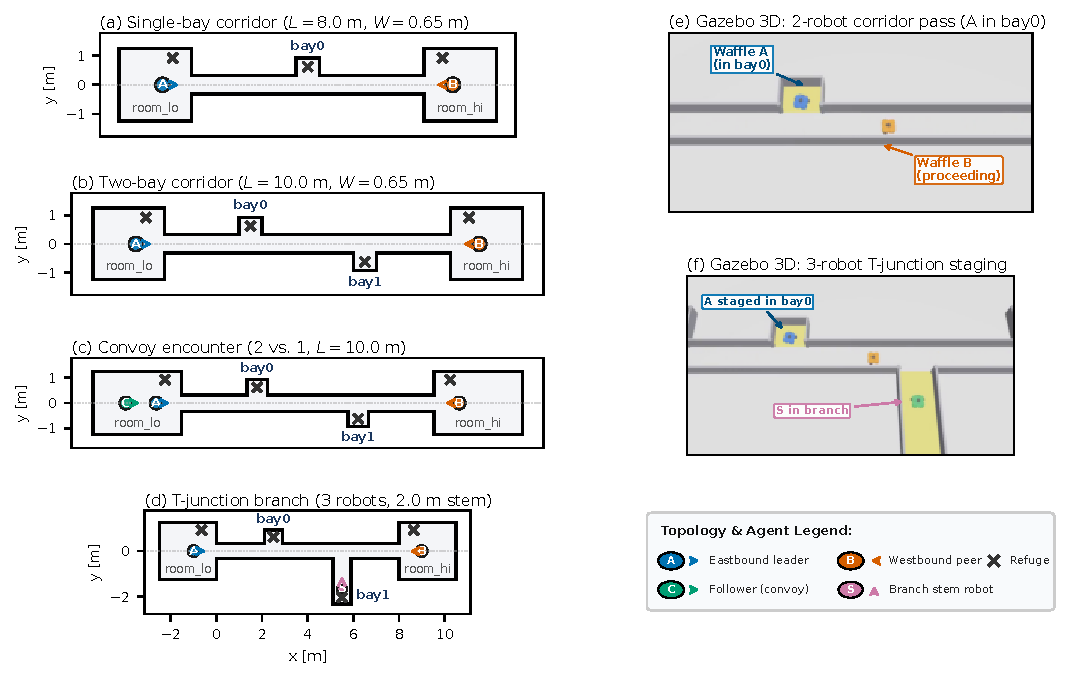
\includegraphics[width=1\textwidth]{Images/scenarios.pdf}
\caption{Benchmark scenario topologies and 3D validation environment. (a)--(d) Top-down 2D layouts (light gray: navigable space; $\times$: discrete refuge parking poses; colored discs/arrows: initial robot poses and travel directions). In (d), the turn-in variant is shown where robot~$S$ starts parked in the branch stem (\texttt{bay1}) and robot~$A$'s destination is \texttt{bay1}; in the exit variant, $A$ and $B$ traverse end-to-end while $S$ exits \texttt{bay1}. (e) Overhead capture from ROS~2 Jazzy / Gazebo Harmonic showing TurtleBot3 Waffle~$A$ parked in \texttt{bay0} while $B$ passes.}
\label{fig:scen}
\end{figure*}
Table~\ref{tab:design} details the complete experimental design across the four research questions (RQ1--RQ4), totaling 18 factorial 2D studies ($50{,}714$ simulated episodes) and 496 seed-paired ROS~2 / Gazebo Harmonic runs (460 main validation runs plus 36 hold-mode runs).

\begin{table*}[!t]\centering
\caption{Complete experimental design grouped by research question. Unless stated otherwise, parameters follow Table~\ref{tab:params}. $N$ counts simulated episodes (each hindsight reference evaluation executes two forced runs).}
\label{tab:design}
{\footnotesize\setlength{\tabcolsep}{3.4pt}
\begin{tabular}{@{}ll>{\raggedright\arraybackslash}p{0.35\textwidth}rlr@{}}\toprule
Layer / RQ & Study (Sec.) & Factorial Grid Factors & Seeds & Policies Evaluated & $N$ \\\midrule
\multirow{6}{*}{RQ1 (Sec.~\ref{sec:rq1})}
 & Single bay (\texttt{S1}) & Bay $x\in\{1,2,3,4,5,6,7\}$\,m & 60 & R, F, D, P, C, O, O$_w$ & 2,940 \\
 & Zone reservation & Bay $x\in\{1,\dots,7\}$\,m (separate 30-seed draw set) & 30 & S, F, D, C, forced A/B & 1,260 \\
 & Two bays (\texttt{S4}) & Bay 1 $\{2,3,4\}\times$ Bay 2 $\{6,7,8\}$\,m $\times$ side; B $U[0,10]$\,s & 20 & R, F, D, P, C, O, O$_w$ & 2,520 \\
 & Asymmetric robots (\texttt{S2}) & $u_B\in\{1,3\}\times$ load $\{0,1\}\times v_B\in\{0.26,0.13\}$\,m/s $\times$ bay $\{2,4,6\}$\,m & 30 & R, F, D, P, C, O, O$_w$ & 5,040 \\
 & Noisy bids (\texttt{S7}) & $\sigma\in\{0,0.1,0.25,0.5,1.0\}\times$ bay $x\in\{1,\dots,7\}$\,m & 30 & C, P, O & 3,150 \\
 & Learned classifier & Train: 800 two-bay pairs; Eval: 150 ID + 150 OOD & -- & L, F, D, C, O$_w$ & 1,600+1,500 \\\midrule
\multirow{3}{*}{RQ2 (Sec.~\ref{sec:rq2})}
 & Unpriced misreport (\texttt{S6}) & B bid scale $k\in\{1,1.5,2,4,10\}\times$ bay $x\in\{2,4,6\}$\,m & 60 & C, O & 1,080 \\
 & Clarke VCG (\texttt{S9}) & Deviator $\{\text{A, B, AB}\}\times 10$ scales $k\in[0.25,4]\times u_B\{1,3\}\times$ bay $\{2,4,6\}$ & 60 & V (+ none/naive eval) & 10,080 \\
 & Repeated fairness (\texttt{S10}) & 50 sequences $\times$ 20 encounters, bay $U[1,7]$\,m; $\lambda\in\{0,0.25,0.5,1,2\}$ & -- & forced A/B (offline) & 2,000 \\\midrule
\multirow{7}{*}{RQ3 (Sec.~\ref{sec:rq3})}
 & Comms sweep (\texttt{S3}) & Loss $\{0,10,30,50,70,90\}\%\times\tau\in\{0.05,0.25,0.5,1,2\}$\,s & 30 & F, D, P, C & 3,600 \\
 & Comms stress (\texttt{S8}) & $R_{\mathrm{det}}\{6,3,1.5\}$\,m $\times v\{0.26,0.5\}$\,m/s $\times$ loss $\{0,50,90\}\%\times\tau\{0.05,0.5,2\}$\,s & 20 & F, D, P, C & 4,320 \\
 & Extreme comms (\texttt{S8b}) & $R_{\mathrm{det}}\in\{1.5,6\}$\,m $\times$ loss $\{90,97,99\}\%\times\tau\in\{2,4,8\}$\,s; $v=0.5$\,m/s & 20 & F, D, P, C & 1,440 \\
 & Safeguard ablation (\texttt{S8c}) & \texttt{S8b} grid $\times$ \texttt{commit} $\{0,1\}\times$ \texttt{state\_guard} $\{0,1\}\times$ \texttt{bay\_check} $\{0,1\}$ & 20 & F, C & 5,760 \\
 & Asymmetric maps & 7 bay-knowledge splits $\times$ \texttt{share\_map} $\{0,1\}\times$ loss $\{0,50\}\%$; bays $3,7$\,m & 10 & F, D, C & 840 \\
 & Blocked bays & Physically obstructed bays $\in\{\emptyset,\text{bay0},\text{bay1},\text{both}\}\times$ loss $\{0,50\}\%$ & 10 & R, F, D, C & 320 \\
 & Explore \& hold & 4 map modes $\times R_{\mathrm{det}}\in\{6,3.5\}$\,m $\times$ loss $\{0,50\}\%$ (+ hold batch) & 30 & F, D, C & 1,440+360 \\\midrule
\multirow{3}{*}{RQ4 (Sec.~\ref{sec:rq4})}
 & Convoy 2 vs.\ 1 & B type (equal, loaded, $u_B=3$) $\times$ bays $\{2,4\}\times\{6,8\}\times$ delay $\{0,4,8\}\times$ loss & 3 & F, D, C, G, side ref. & 1,080 \\
 & T-junction (3 robots) & Delays $(A,B,S)\in\{0,4\}\times\{0,4,8\}\times\{0,6\}$\,s $\times 2$ S goals $\times$ loss $\{0,50\}\%$ & 2 & R, F, D, C & 384 \\
 & ROS~2 / Gazebo 3D & Seed-paired reduced grid across all studies + 36 hold/rerun runs & 6--10 & R, S, F, D, P, L, C, G, V, O & 460+36 \\\bottomrule
\end{tabular}}
\end{table*}

\subsection{Evaluation Metrics, Hindsight Reference, and Statistical Rigor}
Episodes run until all robots reach their goals or the time limit $T_{\max} = 180.0$\,s expires. Each episode records (1)~\emph{success} (all goals reached within 180\,s with zero collisions); (2)~\emph{deadlock} (180\,s reached without collision); (3)~\emph{collision} (SAT overlap of chassis footprints or entering within 0.50\,m of an obstacle); (4)~free-flow-subtracted \emph{delay} $D = \sum_i w_i(T_i - T_i^{\mathrm{free}})$, evaluated unweighted ($w_i = 1$) or urgency-weighted ($w_i = u_i$); (5)~\emph{reverse distance}; and (6)~\emph{first-yielder identity}. (Diagnostic \texttt{min\_clearance} logs axle distance minus $2R_{\mathrm{sw}} = 0.50$\,m, which can turn slightly negative before front bumper contact.)
Because raw delay $D$ conflates policy decision quality with encounter geometry (robots meeting far from any bay incur delay under \emph{any} policy), for every encounter $k$, both forced outcomes, i.e., \texttt{forced\_A} and \texttt{forced\_B}, are simulated, defining the hindsight \emph{best forced yielder} reference $\min(D_A^{(k)}, D_B^{(k)})$. Policy $\pi$'s paired \emph{excess delay} across $N$ encounters is given by
\begin{equation}
\Delta_\pi = \frac{1}{N}\sum_{k=1}^{N}\Bigl(D_\pi^{(k)} - \min\bigl(D_A^{(k)}, D_B^{(k)}\bigr)\Bigr).
\label{eq:excess}
\end{equation}
Here, $\Delta_\pi = 0$ indicates that $\pi$ selected the better yielder on every encounter. Because the reference optimizes only \emph{who} yields under immediate execution, policies that alter conflict timing (e.g., \texttt{hold\_for\_map}) can occasionally achieve $\Delta_\pi < 0$. For 2-vs.-1 convoys, an analogous \texttt{side\_oracle} takes the minimum delay of forcing the convoy vs.\ the lone robot to yield.
All reported statistics reflect the final codebase, apart from explicitly noted pre-fix failure counts that motivated protocol additions. Seed-matched encounters ensure identical start delays and wireless channel noise across all policies. Delays are averaged over successful episodes only, providing a conservative lower bound whenever a policy experiences deadlocks. Uncertainties ($\pm$) denote 95\% confidence intervals (paired per-encounter for $\Delta_\pi$), proportions carry Wilson 95\% intervals, and zero-collision counts report Wilson 95\% upper bounds.